%  LaTeX support: latex@mdpi.com
%  In case you need support, please attach any log files that you could have, and specify the details of your LaTeX setup (which operating system and LaTeX version / tools you are using).

%=================================================================

% LaTeX Class File and Rendering Mode (choose one)
% You will need to save the "mdpi.cls" and "mdpi.bst" files into the same folder as this template file.

%=================================================================

\documentclass[journal,article,accept,moreauthors,pdftex,12pt,a4paper]{mdpi} 
\usepackage{tikz}
\usepackage{tikz-3dplot}
\usetikzlibrary{shapes,calc,positioning}
\tdplotsetmaincoords{60}{60}
\usepackage{amsmath}
\usepackage{graphicx,subcaption}

%--------------------
% Class Options:
%--------------------
% journal
%----------
% Choose between the following MDPI journals:
% actuators, administrativesciences, aerospace, agriculture, agronomy, algorithms, animals, antibiotics, antibodies, antioxidants, appliedsciences, arts, atmosphere, atoms, axioms, batteries, behavioralsciences, bioengineering, biology, biomedicines, biomolecules, biosensors, brainsciences, buildings, cancers, catalysts, cells, challenges, chemosensors, children, chromatography, climate, coatings, computation, computers, cosmetics, crystals, dentistryjournal, diagnostics, diseases, diversity, econometrics, economies, education, electronics, energies, entropy, environmentalsciences, environments, epigenomes, fibers, foods, forests, futureinternet, galaxies, games, gels, genealogy, genes, geosciences, healthcare, horticulturae, humanities, hydrology, informatics, information, inorganics, insects, ijerph, ijfs, ijms, ijgi, jcdd, jcm, jdb, jfb, jimaging, jof, joi, jlpea, jmse, jpm, jrfm, jsan, land, laws, life, lubricants, machines, marinedrugs, materials, mathematics, medicalsciences, membranes, metabolites, metals, microarrays, micromachines, microorganisms, minerals, molbank, molecules, nanomaterials, ncrna, nutrients, pathogens, pharmaceuticals, pharmaceutics, pharmacy, photonics, plants, polymers, processes, proteomes, publications, religions, remotesensing, resources, risks, robotics, safety, sensors, sinusitis, socialsciences, societies, sports, standards, sustainability, symmetry, systems, technologies, toxics, toxins, universe, vaccines, veterinarysciences, viruses, water
%---------
% article
%---------
% The default type of manuscript is article, but could be replaced by using one of the class options: 
% article, review, communication, commentary, bookreview, correction, addendum, editorial, changes, supfile, casereport, comment, conceptpaper, conferencereport, meetingreport, discussion, essay, letter, newbookreceived, opinion, projectreport, reply, retraction, shortnote, technicalnote, creative
%----------
% submit
%----------
% The class option "submit" will be changed to "accept" by the Editorial Office when the paper is accepted. This will only make changes to the frontpage (e.g. the logo of the journal will get visible), the headings, and the copyright information. Journal info and pagination for accepted papers will also be assigned by the Editorial Office.
% Please insert a blank line is before and after all equation and eqnarray environments to ensure proper line numbering when option submit is chosen
%------------------
% moreauthors
%------------------
% If there is only one author the class option oneauthor should be used. Otherwise use the class option moreauthors.
%---------
% pdftex
%---------
% The option "pdftex" is for use with pdfLaTeX only. If eps figure are used, use the optioin "dvipdfm", with LaTeX and dvi2pdf only.

%=================================================================
\setcounter{page}{1}
\lastpage{x}
\doinum{10.3390/------}
\pubvolume{xx}
\pubyear{2015}
%\externaleditor{Academic Editor: xx}
\history{Received: xx / Accepted: xx / Published: xx}
%------------------------------------------------------------------
% The following line should be uncommented if the LaTeX file is uploaded to arXiv.org
%\pdfoutput=1

%=================================================================

% Add packages and commands to include here
% The amsmath, amsthm, amssymb, hyperref, caption, float and color packages are loaded by the MDPI class.
%\usepackage{graphicx}
%\usepackage{subfigure,psfig}

%=================================================================
%% Please use the following mathematics environments:
%\theoremstyle{mdpi}
%\newcounter{thm}
%\setcounter{thm}{0}
%\newcounter{ex}
%\setcounter{ex}{0}
%\newcounter{re}
%\setcounter{re}{0}
%\newtheorem{Theorem}[thm]{Theorem}
%\newtheorem{Lemma}[thm]{Lemma}
%\newtheorem{Characterization}[thm]{Characterization}
%\newtheorem{Proposition}[thm]{Proposition}
%\newtheorem{Property}[thm]{Property}
%\newtheorem{Problem}[thm]{Problem}
%\newtheorem{Example}[ex]{Example}
%\newtheorem{Remark}[re]{Remark}
%\newtheorem{Corollary}[thm]{Corollary}
%\newtheorem{Definition}[thm]{Definition}
%% For proofs, please use the proof environment (the amsthm package is loaded by the MDPI class).

%=================================================================

% Full title of the paper (Capitalized)
\Title{Comparing probabilistic predictive models applied to football}

% Authors (Add full first names)
\Author{Marcio A. Diniz $^{1,}$*, Rafael Izbicki $^{1}$, Danilo Lopes $^{1}$ and Luis Ernesto Salasar $^{1}$}

% Affiliations / Addresses (Add [1] after \address if there is only one affiliation.)
\address{%
$^{1}$ Department of Statistics, Federal University of S\~ao Carlos, Rod. Washington Luis, km 235, S. Carlos, Brazil}

% Contact information of the corresponding author (Add [2] after \corres if there are more than one corresponding author.)
\corres{e-mail, telephone and fax number of the corresponding author.}

% Abstract (Do not use inserted blank lines, i.e. \\) 
\abstract{This is the abstract section. The abstract should be one section and count less than 200 words.}

% Keywords: add 3 to 10 keywords
\keyword{keyword; keyword; keyword}

% The fields PACS, MSC, and JEL may be left empty or commented out if not applicable
%\PACS{}
%\MSC{}
%\JEL{}

% If this is an expanded version of a conference paper, please cite it here: enter the full citation of your conference paper, and add $^\dagger$ in the end of the title of this article.
%\conference{}

\begin{document}

%%%%%%%%%%%%%%%%%%%%%%%%%%%%%%%%%%%%%%%%%%

\section{Introduction}

The famous saying of John von Neumann: {\it ``With four parameters I can fit an elephant, and with five I can make him wiggle his trunk''} is a perhaps just a humorous version of Ockham's razor: 
{\it``Entities are not to be multiplied without necessity''}, but illustrates very well a principle that is not often followed by researchers, especially when building predictive models. 
This is true also in the literature of probabilistic sports predictions, particularly regarding models devoted to football predictions.

Bothered by such concerns, our goal was to answer the following question: is it possible, using a simple probabilistic model, to predict results of football matches better than more sophisticated or complex models?
To answer this, we compared two sophisticated models with simple multinomial-Dirichlet models that consider only the number of matches won, drawn or lost by each team as inputs.
The models were tested for the second round of the Brazilian football championships of first and second divisions and compared using standard metrics or scoring rules.
We also used other criteria such as the proportion of matches that were predicted ``correctly'' by each model and a measure of calibration, both explained in detail below.
According to the adopted criteria, the simple models showed a similar predictive performance to the complex ones.

The predictions of the complex models used here as benchmarks are published on Internet websites for every matchday, and are treated by us as black-box models since we are not interested in how they were built or the assumptions on which they are based.
We know that\footnote{One of the authors is responsible for one of these models and the other was described in a dissertation.} both models are based on the bivariate Poisson or Holgate distribution, being able to predict the final score of a match given explanatory variables.
\footnote{For more details see \cite{arruda2000}.}
Therefore, to estimate the probability that, for instance, the home team will win, the estimated model---the model estimated with available information---is simulated a given number of times and the proportion of simulated scores favoring the home team will be the predicted probability of the model.
Knowing that both models are based on an elaborate parametric model, they are suitable for the comparison we are proposing: simple versus complex models.

There are several ways to score or classify predictions of categorical events that assume one out of three possible outcomes, like football matches.
See \cite{constantinou} for a brief survey of such measures applied to football.
We decided to score the previsions for each match in terms of their distances from the truth, i.e. the verified event, once it has occurred, and chose the most used distances in the literature: Brier (\cite{brier1950}), logarithmic and spherical.
The total inaccuracy of each model is then defined as the sum of the point-wise scores of all its previsions.

This paper is organized as follows.
Section 1 describes the proposed models, Section 2 presents the scoring rules and criteria used in this work to classify the models.
Section 3 reports the performance of the models predicting 380 matches comprising the second half of Brazilian championships of first and second divisions.
In Section 4 we discuss the results, and Section 5 closes with some remarks and proposals for future research.




%%%%%%%%%%%%%%%%%%%%%%%%%%%%%%%%%%%%%%%%%%

\section{Experimental Section}
%% Only for the journal Gels: Please place the Experimental Section after the Conclusions

The black-box models used as benchmarks make their predictions available at {chancedegol.uol.com.br} and {www.previsaoesportiva.com.br}.

%%%%%%%%%%%%%%%%%%%%%%%%%%%%%%%%%%%%%%%%%%

\subsection{Multinomial-Dirichlet}

Considering team $A$: the result of its next match may be considered a categorical random quantity (r.q.) that may assume only three modes; win ($W$), draw ($D$) or loss ($L$).

it is all wrong.

If we denote the probability of $W$, by $\theta_1$, of $D$ by $\theta_2$ and of $L$ by $\theta_3=1-\theta_1-\theta_2$ where $\theta_1+\theta_2\leq 1$.

The p.m.f of such r.q. is

\[
P(X=x|\theta)=\theta_1^{I(x=W)}\theta_2^{I(x=D)}(1-\theta_1-\theta_2)^{I(x=L)}
\]

\noindent
where $\mathcal{X}=\{W,D,L\}$ and $I(x=i)$ is the indicator function, that takes value 1 if $x$ equals $i= W, D, L$ and 0 otherwise; $\theta=\{(\theta_1,\theta_2)\in\Re^2:\theta_1+\theta_2\leq1 ~ \text{and} ~ \theta_i\geq0 ~ \text{for} ~ i=1, 2\}$

We may also call it multivariate Bernoulli r.q.

Assuming that the matches of team $A$, given $\theta$, are i.i.d. with categorical distribution, the sum of $n$ r.q.'s has multinomial distribution with parameters $\theta$ and $n$.

\[
P(M_1=n_1,M_2=n_2,M_3=n_3|\theta,n)=\]
\[
\frac{n!}{n_1!n_2!(n-n_1-n_2)!}\theta_1^{n_1}\theta_2^{n_2}(1-\theta_1-\theta_2)^{n-n_1-n_2}
\]

when $n_1+n_2+n_3=n$ and 0 otherwise, for non-negative integers $n_1$, $n_2$ and $n_3$.

$n_1$ is the number of matches won, $n_2$ the matches drawn and $n_3=n-n_1-n_2$ the matches lost.

{\bf Summary}: under the given assumptions, the vector of matches won, drawn or lost by some team, has multinomial distribution with parameters $n$ and $\theta$.

Our goal is to compute: 

\[P(X_{n+1}=W|M_1=n_1,M_2=n_2,M_3=n_3)=p_1;\]

\[P(X_{n+1}=D|M_1=n_1,M_2=n_2,M_3=n_3)=p_2;\] and

\[P(X_{n+1}=L|M_1=n_1,M_2=n_2,M_3=n_3)=p_3.\]


Using Bayesian inference these probabilities are easily computed: if the prior for $\theta$ is Dirichlet with parameter vector $(\alpha_1,\alpha_2,\alpha_3)$, i.e. its density function is

\[
f(\theta|\alpha)=\frac{\Gamma(\alpha_1+\alpha_2+\alpha_3)}{\Gamma(\alpha_1)\Gamma(\alpha_2)\Gamma(\alpha_3)}\theta_1^{\alpha_1-1}\theta_2^{\alpha_2-1}(1-\theta_1-\theta_2)^{\alpha_3-1}
\]

\noindent
for $\alpha_1$, $\alpha_2$, $\alpha_3 > 0$, then the posterior is Dirichlet with parameters $(n_1+\alpha_1,n_2+\alpha_2,n_3+\alpha_3)$, and hence

\[p_1=P(X_{n+1}=W|M_1=n_1,M_2=n_2,M_3=n_3)=\frac{n_1+\alpha_1}{n+\alpha};\]

\noindent
where $n=n_1+n_2+n_3$ and $\alpha=\alpha_1+\alpha_2+\alpha_3$.

Similarly

\[p_2=P(X_{n+1}=D|M_1=n_1,M_2=n_2,M_3=n_3)=\frac{n_2+\alpha_2}{n+\alpha};\]

\[p_3=P(X_{n+1}=L|M_1=n_1,M_2=n_2,M_3=n_3)=\frac{n_3+\alpha_3}{n+\alpha};\]

Parameters of the prior: (1,1,1), uniform on the simplex.

\section{Scoring rules and calibration}

How can we fairly distinguish better-informed states of knowledge from more poorly informed states?
Using proper scoring rules for evaluating states of uncertain knowledge.
A scoring rule is a function of two variables (or vectors, matrices etc) that accords a real number (score) to each pair of numbers that could represent the value of X and the prevision value, P(X).
It is maximum for each x when x=P(X) and nonincreasing as x departs from P(X) for each P(X), and as P(X) departs from x for each x.
The best score is achieved when knowledge of X is asserted as the value of X itself, whatever it might be.
Most of the scoring rules exhibit an arbitrary normalizing feature, that S[x,P(X)]=0 for each x.
Many functions satisfy the criteria for a scoring rule specified above, but not every scoring rule would be regarded as providing a fair assessment of the assertion P(X).
Proper scoring rules encourages honesty and accuracy in assessing numerical values for their previsions.

One usage of a scoring function could be to give a reward of $S(\mathbf{r},i)$ if the ith event occurs. If a proper scoring rule is used, then the highest expected reward is obtained by reporting the true probability distribution. The use of a proper scoring rule encourages the forecaster to be honest to maximize the expected reward.

The scoring rule is constructed according to the basic idea that the resulting device should oblige each participant to express his true feelings, because any departure from his own personal probability results in a diminution of his own average score as he sees it.

Moreover, this method leads automatically to an overall comparison between the outcomes of different personal evaluations concerned with the same totality of events.
The accumulated loss is indeed a throughly concrete measure of success.

Proper scoring rules are devised so that no one previses (expects) that intrigue in falsely announcing some other number as P(X) would be advantageous for achieving a better score.
The particular scoring functions we study in the generic form S(X,P(X)) can also be considered as utility functions, U(X,P(X)).
The principle of asserting numerical values for P(X) in such a way as to maximize your prevision for your score is equivalent to acting in a decision problem so as to maximize your expected utility.

Probability assertions are said to be well calibrated at the level of probability p if the observed proportion of all propositions that are assessed with probability p equals p.

A person's probability assertions are said to be well calibrated at the value p if the limiting frequency of occurrence of events that are assessed with probability p, equals p.

\subsection{Brier score}

\begin{figure}
\begin{center}
\begin{tikzpicture}[scale=2,tdplot_main_coords,axis/.style={->},thick]

% -- remove these 3 lines if no axis is preferred
\draw[axis] (0, 0, 0) -- (1.4, 0, 0) node [right] {$p_1$};
\draw[axis] (0, 0, 0) -- (0, 1.4, 0) node [above] {$p_2$};
\draw[axis] (0, 0, 0) -- (0, 0, 1.4) node [above] {$p_3$};

\coordinate  (d1) at (1,0,0){};
\coordinate  (d2) at (0,1,0){};
\coordinate  (d3) at (0,0,1){};

% fill gray color with opacity
\fill[green!80,opacity=0.2] (d1) -- (d2) -- (d3)-- cycle;

\draw[-, green, thick] (0,0,1) -- (1,0,0);
\draw[-, green, thick] (0,0,1) -- (0,1,0);
\draw[-, green ,thick] (1,0,0) -- (0,1,0);

\node[fill,circle,inner sep=1.5pt,label={left:$(1,0,0)$}] at (d1) {};
\node[fill,circle,inner sep=1.5pt,label={south east:$(0,1,0)$}] at (d2) {};
\node[fill,circle,inner sep=1.5pt,label={left:$(0,0,1)$}] at (d3) {};

\draw[-latex,thick](d3) to [out=60,in=180] (1,1,2);

\node[label={right:away team wins}] at (1,1,2) {};

\draw[-latex,thick](d1) to [out=-90,in=180] (1,1,-1);

\node[label={right:home team wins}] at (1,1,-1) {};

\draw[-latex,thick](d2) to [out=-120,in=180] (1,1,-.25);

\node[label={right:draw}] at (1,1,-.25) {};

\node[fill, blue, circle,inner sep=1.5pt] at (0.25,0.35,0.40) {};

\draw[-latex,thick](0.25,0.35,0.40) to [out=90,in=180] (1,1,1.2);

\node[label={right:$(0.25,0.35,0.40)$: prediction}] at (1,.9,1.2) {};

\end{tikzpicture}
\caption{Bi-dimensional simplex (green surface): area of possible predictions}\label{fig:simplex}
\end{center}
\end{figure}

The green surface represents the 2-simplex, i.e. the set of points such that $p_1+p_2+p_3=1$ for non-negative values of $p_1$, $p_2$ and $p_3$.
The triangle representing the simplex has sides of length $\sqrt{2}$ and its height is $\sqrt{6}/2$.
Drawing a similar equilateral triangle with height 1 and sides $2\sqrt{3}/3$, it is possible to represent all the points of the simplex.
This new triangle is usually used to graphically display the predictions as internal points because the sum of the distances of every point inside it to each side is always one representing the probability of each event.

\begin{figure}[!ht]
    \centering
    \begin{subfigure}[b]{0.48\linewidth}        %% or \columnwidth
        \centering

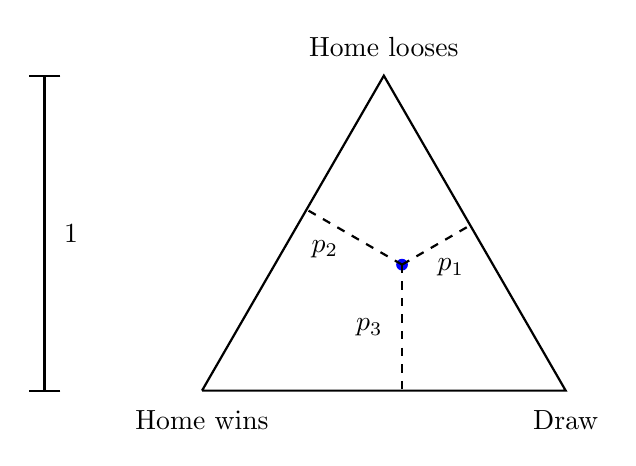
\begin{tikzpicture}[scale=4]
\draw [thick](0,0) -- (1.1547,0) -- (0.57735,1)-- (0,0);

\node[fill, blue, circle,inner sep=1.5pt] at (0.63509,0.40) {};

\draw[dashed,thick] (0.63509,0.40) -- (0.63509,0);
\draw[dashed,thick] (0.63509,0.40) -- (0.85159,0.525);
\draw[dashed,thick] (0.63509,0.40) -- (0.331976,0.575);

\node[label={left:$p_3$}] at (.63509,.2) {};
\node[label={below:$p_1$}] at (.79,.48) {};
\node[label={below:$p_2$}] at (.39,.54) {};

\node[label={below:Home wins}] at (0,0) {};
\node[label={below:Draw}] at (1.1547,0) {};
\node[label={above:Home looses}] at (0.57735,1) {};


\draw[-,thick] (-.5,0) -- (-.5,1);
\draw[-,thick] (-.45,0) -- (-.55,0);
\draw[-,thick] (-.45,1) -- (-.55,1);

\node[label={right:$1$}] at (-.5,.5) {};


\end{tikzpicture}


        \caption{Normalized simplex: $p_1+p_2+p_3=1$}
        \label{fig:A}
    \end{subfigure}
    \begin{subfigure}[b]{0.48\linewidth}        %% or \columnwidth
        \centering

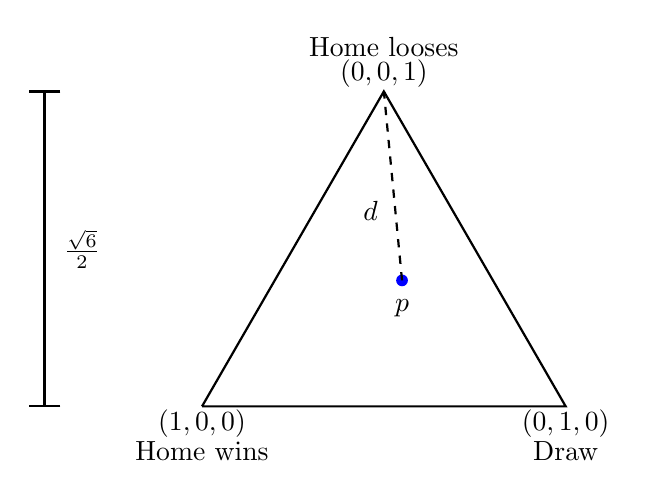
\begin{tikzpicture}[scale=4]
\draw [thick](0,0) -- (1.1547,0) -- (0.57735,1)-- (0,0);

\node[fill, blue, circle,inner sep=1.5pt] at (0.63509,0.40) {};
\node[label={below:$p$}] at (0.63509,0.40) {};

\node[label={left:$d$}] at (0.62,0.62) {};


\draw[dashed,thick] (0.63509,0.40) -- (0.57735,1);

\node[label={below:Home wins}] at (0,-0.05) {};
\node[label={below:Draw}] at (1.1547,-0.05) {};
\node[label={above:Home looses}] at (0.57735,1.05) {};

\node[label={below:$(1,0,0)$}] at (0,0.05) {};
\node[label={below:$(0,1,0)$}] at (1.1547,0.05) {};
\node[label={above:$(0,0,1)$}] at (0.57735,0.95) {};


\draw[-,thick] (-.5,0) -- (-.5,1);
\draw[-,thick] (-.45,0) -- (-.55,0);
\draw[-,thick] (-.45,1) -- (-.55,1);

\node[label={right:$\frac{\sqrt{6}}{2}$}] at (-.5,.5) {};

\end{tikzpicture}


        \caption{Original simplex: used to compute the Brier score}
        \label{fig:B}
    \end{subfigure}
    \caption{Normalized and standard simplexes}
    \label{fig:norm_stand}
\end{figure}



For every point inside this triangle $p_1+p_2+p_3=1$.



\[p=(0.25,0.35,0.40)\]
\[d^2=(0-0.25)^2+(0-0.35)^2+(1-0.40)^2=0.545\]

%%%%%%%%%%%%%%%%%%%%%%%%%%%%%%%%%%%%%%%%%%

\section{Example}

Gr\^emio $\times$ Atl\'etico-PR (Matchday 20), at Gr\^emio.

\begin{table}[h]
\begin{center}
\begin{tabular}{lccccccccc}

\hline
 & \multicolumn{3}{c}{Home} & \multicolumn{3}{c}{Away}& \multicolumn{3}{c}{Overall} \\
\hline
\hline
Team & W & D & L & W & D & L & W & D & L\\
\hline
Gr\^emio & 6 & 2 & 1 & 3 & 2 & 5 & 9 & 4 & 6\\
Atl\'etico-PR & 4 & 4 & 2 & 2 & 3 & 4 & 6 & 7 & 6\\
\hline
\end{tabular}
\caption{Gr\^emio and Atl\'etico-PR counts after 19 matchdays (first round)}
\end{center}
\end{table}



$h_1$=number of matches won by Gr\^emio when playing home

$h_2$=number of matches drawn by Gr\^emio when playing home

$h_3$=number of matches lost by Gr\^emio when playing home

\

$(h_1,h_2,h_3)=(6,2,1)$


\[
p_{1h}=\frac{h_1+\alpha_1}{h+\alpha}=\frac{6+1}{9+3}=\frac{7}{12}=0.583\]

\[
p_{2h}=\frac{h_2+\alpha_2}{h+\alpha}=\frac{2+1}{9+3}=\frac{3}{12}=0.25\]

\[
p_{3h}=\frac{h_3+\alpha_3}{h+\alpha}=\frac{1+1}{9+3}=\frac{2}{12}=0.167\]


$a_1$=number of matches won by Atl\'etico-PR when playing away

$a_2$=number of matches drawn by Atl\'etico-PR when playing away

$a_3$=number of matches lost by Atl\'etico-PR when playing away

\

$(a_1,a_2,a_3)=(3,2,5)$


\[
p_{1a}=\frac{a_1+\alpha_1}{h+\alpha}=\frac{2+1}{9+3}=\frac{3}{12}=0.25\]

\[
p_{2a}=\frac{a_2+\alpha_2}{h+\alpha}=\frac{3+1}{9+3}=\frac{4}{12}=0.333\]

\[
p_{3a}=\frac{a_3+\alpha_3}{h+\alpha}=\frac{4+1}{9+3}=\frac{5}{12}=0.417\]


What's the probability that Gr\^emio wins: $p_{1h}=0.583$ or $p_{3a}=0.417$?

What's the probability of a draw: $p_{2h}=0.25$ or $p_{2a}=0.333$?

What's the probability that Gr\^emio looses: $p_{3h}=0.167$ or $p_{1a}=0.25$?


Three ways of combining these probabilities are proposed: (I) a mixture with equal weights to both teams; 

\[
\frac{1}{2}\times p_{1h}+\frac{1}{2}\times p_{3a}=\frac{1}{2}\times0.583+\frac{1}{2}\times0.417=0.5
\]

\noindent
is the probability that Gr\^emio wins.


\[
\frac{1}{2}\times p_{2h}+\frac{1}{2}\times p_{2a}=\frac{1}{2}\times0.25+\frac{1}{2}\times0.333=0.2917
\]

\noindent
is the probability of a draw.

\[
\frac{1}{2}\times p_{3h}+\frac{1}{2}\times p_{1a}=\frac{1}{2}\times0.167+\frac{1}{2}\times0.25=0.2083
\]

\noindent
is the probability that Atl\'etico wins.


(II) a mixture with weights (inversely) proportional to the teams rank before the match; 
after 19 matchdays, Gr\^emio was the $6^{th}$ place and Atl\'etico-PR the $11^{th}$:


\[w_1 = \frac{1/6}{1/6+1/11}=0.647 ~ ~ ~ ~ ~ w_2 = \frac{1/11}{1/6+1/11}=0.353\]


\[
w_1\times p_{1h}+w_2\times p_{3a}=0.647\times0.583+0.353\times0.417=0.525 (\text{Gr\^emio wins})
\]

\[
w_1\times p_{2h}+w_2\times p_{2a}=0.647\times0.25+0.353\times0.333=0.279 (\text{draw})
\]

\[
w_1\times p_{1h}+w_2\times p_{3a}=0.647\times0.167+0.353\times0.25=0.196 (\text{Atl\'etico wins})
\]
    

(III) combine the counts to generate one prediction: 

$(h_1,h_2,h_3)=(6,2,1)$ and $(a_1,a_2,a_3)=(2,3,4)$ $\Rightarrow$ $(c_1,c_2,c_3)=(10,5,3)$


$c_1=h_1+a_3 \Rightarrow$ number of matches won by Gr\^emio playing home plus matches lost by Atl\'etico playing away.

\[\frac{c_1+\alpha_1}{c+\alpha}=\frac{10+1}{18+3}=0.524
\] 


\[\frac{c_2+\alpha_3}{c+\alpha}=\frac{5+1}{18+3}=0.286
\] 

\[\frac{c_3+\alpha_3}{c+\alpha}=\frac{3+1}{18+3}=0.190
\] 

\noindent
where $c=c_1+c_2+c_3$, $c_2=h_2+a_2$ and $c_3=h_3+a_1$.

Final result: Gr\^emio 1 $\times$ 0 Atl\'etico-PR

\begin{table}[h]
\begin{center}
\begin{tabular}{ccccc}

\hline
Model & Gr\^emio & Draw & Atl\'etico-PR & Score \\
\hline
\hline
BB1 & 0.505 & 0.263 & 0.232 & 0.368 \\
BB2 & 0.55 & 0.27 & 0.18 & 0.308 \\
$Mn-Dir_1$ & 0.50 & 0.292 & 0.208 & 0.379 \\
$Mn-Dir_2$ & 0.525 & 0.279 & 0.196 & 0.342\\
$Mn-Dir_3$ & 0.524 & 0.286 & 0.190 & 0.345\\
\hline
\end{tabular}
%\caption{Score of the ten first rounds and mean score per match after 190 matches}
\end{center}
\end{table}


\section{Results}

\subsection{First Division (S\'erie A)}

\begin{table}[h]
\begin{center}
\begin{tabular}{cccccc}

\hline
Matchday & BB1 & BB2 & $Mn-Dir_1$ & $Mn-Dir_2$ & $Mn-Dir_3$\\
\hline
\hline
1$^{st}$ &4.992 & 5.055 & 5.630 & 5.053 & 5.521 \\
2$^{nd}$ &5.006 & 5.328 & 5.327 & 5.533 & 5.201 \\
3$^{rd}$ &7.129 & 6.568 & 7.979 & 7.640 & 8.216 \\
4$^{th}$ &5.941 & 5.782 & 6.513 & 6.848 & 6.564 \\
5$^{th}$ &5.246 & 5.858 & 5.669 & 5.368 & 5.601 \\
6$^{th}$ &5.584 & 5.095 & 6.055 & 6.112 & 6.033 \\
7$^{th}$ &5.641 & 5.817 & 5.250 & 5.062 & 5.134 \\
8$^{th}$ &6.112 & 6.710 & 6.315 & 6.673 & 6.348 \\
9$^{th}$ &6.433 & 6.714 & 5.768 & 6.061 & 5.717 \\
10$^{th}$ &4.912 & 4.620 & 6.019 & 6.115 & 6.010 \\
\hline
Total & 111.04 & 111.32 & 115.45 & 115.36 & 115.29 \\
\hline
Mean & 0.5844 & 0.5859 & 0.6076 & 0.6072 & 0.6068 \\
\hline
\end{tabular}
\caption{Score of the ten first rounds and mean score per match after 190 matches}
\end{center}
\end{table}


\subsection{Second Division (S\'erie B)}

\begin{table}[h]
\begin{center}
\begin{tabular}{ccccc}

\hline
Matchday & BB1 & $Mn-Dir_1$ & $Mn-Dir_2$ & $Mn-Dir_3$\\
\hline
\hline
1$^{st}$ & 7.267 & 8.003 & 8.131 & 8.263 \\
2$^{nd}$ & 5.633 & 6.073 & 6.119 & 6.057 \\
3$^{rd}$ & 7.183 & 7.086 & 7.384 & 7.183 \\
4$^{th}$ & 7.458 & 6.776 & 6.731 & 6.829 \\
5$^{th}$ & 5.246 & 5.492 & 5.494 & 5.414 \\
6$^{th}$ & 5.126 & 5.169 & 5.589 & 5.043 \\
7$^{th}$ & 5.837 & 5.033 & 4.939 & 4.897 \\
8$^{th}$ & 7.462 & 6.616 & 6.509 & 6.667 \\
9$^{th}$ & 8.223 & 7.520 & 7.733 & 7.671 \\
10$^{th}$ & 4.818 & 5.623 & 5.825 & 5.578 \\
\hline
Total & 118.00 & 117.68 & 119.33 & 117.70 \\
\hline
Mean & 0.6178 & 0.6161 & 0.6248 & 0.6162 \\

\hline
\end{tabular}
\caption{Score of the ten first rounds and mean score per match after 191 matches}
\end{center}
\end{table}


\begin{table}[h]
\begin{center}
\begin{tabular}{ccccc}

\hline
BB1 & $Mn-Dir_1$ & $Mn-Dir_2$ & $Mn-Dir_3$\\
\hline
\hline
0.6011 & 0.6119 & 0.6159 & 0.6115\\
\hline
\multicolumn{4}{c}{Chance de gol historic mean (1998-2015): 0.5977}\\
\hline
\end{tabular}
\caption{First and Second Divisions means}
\end{center}
\end{table}

\section{Discussion}
%De Finetti was a radical subjectivist and pragmatist about probability and did not believe that it even made sense to talk about credences as being ``accurate'' or ``inaccurate''. 
%Like Ramsey and Savage, he offered pragmatic arguments for probabilism. 
%As a result, de Finetti did not speak of ``measures of inaccuracy'' or ``measures of distance from the truth'': he used the terms ``scoring rule'' and ``loss function''.


%De Finetti used what is called the Brier score, which is just the (squared) Euclidean distance — i.e., the sum of the squared differences between credences and (the 0/1 numerical correlates of) truth values.

It is possible to interpret the score as a numerical measure of how inaccurate was the 
prevision. 


%%%%%%%%%%%%%%%%%%%%%%%%%%%%%%%%%%%%%%%%%%

\section{Conclusions}

We compared the probabilistic predictions of three simple models with the ones provided by two more complex models for the second round of the 2014 Brazilian football championships of first and second divisions.
According to standard scoring rules and other criteria here adopted to qualify the predictions, our results show that the predictive power of all models was quite similar.

On the one hand, our findings appear as another supportive example of Ockham's razor but, on the other, poses several questions about probabilistic prediction of sport events.
We mention just a couple of them, raised by the similar performance of the considered models: is there an irreducible ``randomness'' or ``degree of unpredictability'' implicit in these events?
Is this degree an indicator of how close is the championship being studied?
To answer these questions we would have to consider more championships and models and compare them using other scoring rules, being a suggestion for further research.
Also as future research we would like to test other weights and study their impact on the predictive power of models 1 and 2 here proposed.


%The most useful statement of the principle for scientists is
%"when you have two competing theories that make exactly the same predictions, the simpler one is the better."

%What to infer from known recorded measurements about the values of yet unrecorded measurements is the responsibility of each knowing person.
%There is general agreement in evaluating the evidence that the measured observations provide for yet unmeasured experiences.
%There have been controversies among very respected scientists regarding what conclusions are to be drawn from observations.



%%%%%%%%%%%%%%%%%%%%%%%%%%%%%%%%%%%%%%%%%%

\acknowledgments{Acknowledgments}

Main text.

%%%%%%%%%%%%%%%%%%%%%%%%%%%%%%%%%%%%%%%%%%

\authorcontributions{Author Contributions}

Main text.

%%%%%%%%%%%%%%%%%%%%%%%%%%%%%%%%%%%%%%%%%%

\conflictofinterests{Conflicts of Interest}

State any potential conflicts of interest here or ``The authors declare no conflict of interest''. 

%=================================================================
% References: Variant A
%=================================================================
% Back Matter (References and Notes)
%----------------------------------------------------------
% Style and layout of the references
\bibliographystyle{mdpi}
\makeatletter
\renewcommand\@biblabel[1]{#1. }
\makeatother

\begin{thebibliography}{999} % if there are less than 10 entries, enter a one digit number

% Reference 1
\bibitem{ref-journal}
Lastname, F.; Author, T. The title of the cited article. {\em Journal Abbreviation} {\bf 2008}, {\em 10}, 142-149.

% Reference 2
\bibitem{ref-book}
Lastname, F.F.; Author, T. The title of the cited contribution. In {\em The Book Title}; Editor, F., Meditor, A., Eds.; Publishing House: City, Country, 2007; pp. 32-58.


\bibitem{arruda2000}
Arruda, M. L. {\em Poisson, Bayes, Futebol e De Finetti}, M. A. dissertation (in Portuguese), University of S\~ao Paulo, 2000.

\bibitem{brier1950}
Brier, G. Verification of forecasts expressed in terms of probability. {\em Monthly Weather Review} {\bf 1950}, {\em 78}, 1-3.

\bibitem{constantinou}
Constantinou, A. and Fenton, N. E. Evaluating the Predictive Accuracy of Association Football Forecasting Systems. Unpublished paper.


\end{thebibliography}

%=================================================================
% References:  Variant B
%=================================================================
% Use the following option to include external BibTeX files:
%\bibliography{lite}
%\bibliographystyle{mdpi}

%%%%%%%%%%%%%%%%%%%%%%%%%%%%%%%%%%%%%%%%%%

%\abbreviations{Abbreviations/Nomenclature}
%
%Main text.

%%%%%%%%%%%%%%%%%%%%%%%%%%%%%%%%%%%%%%%%%%

%\appendix
%\section{Appendix Title}
%
%Main text.

\end{document}

